\chapter{Modèle Particle-Over-Particle }
    \label{chap-pop}


%%%%%%%%%%%%%%%%%%%%%%%%%%%%%
	\section{Modèle de particules : le modèle POP}
%%%%%%%%%%%%%%%%%%%%%%%%%%%%%


\begin{figure}
    \centering
    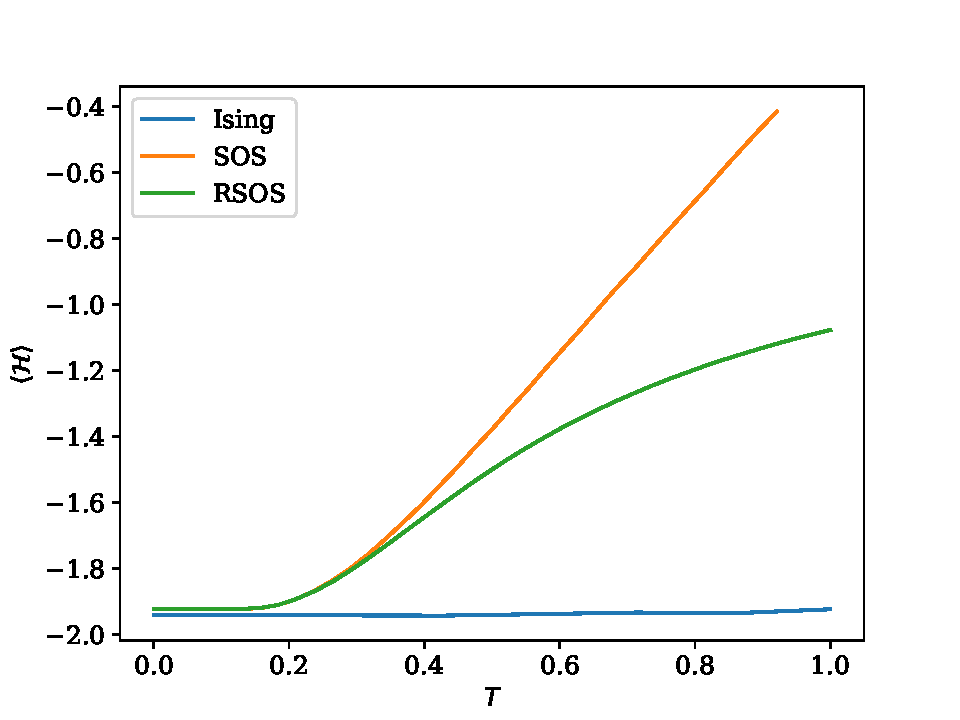
\includegraphics[width=0.5\textwidth]{isingtosos/comparaison-modeles.pdf}
    \caption{Énergie par site entre les modèles d'Ising (\ref{hamil-ising}) (avec conditions fixes en $y$), SOS et RSOS (\ref{hamil-sos}) et POP (\ref{hamil-pop}) en fonction de la température via des simulations de Monte Carlo pour $L_X=64$, $L_Y=51$ et $J=1$ avec des conditions périodiques en $x$. La configuration intiale est la configuration à $T=0$ d'une interface parfaitement lisse. {\color{red} Besoin refaire Ising avec MCIA. et ajouter $J\to2J$ dans la simu pour SOS} }
    \label{comparaison-modeles}
\end{figure}

\begin{figure}[h]
	\centering
	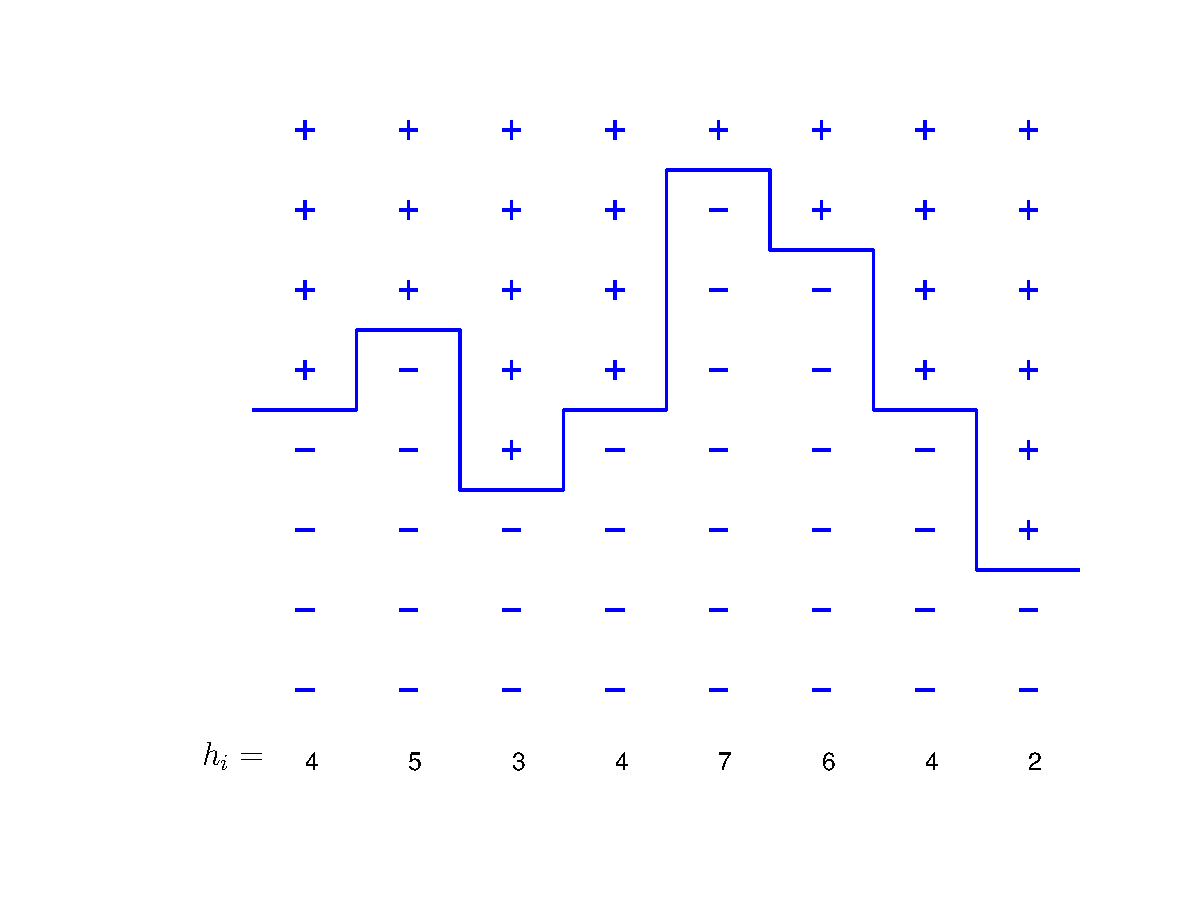
\includegraphics[width=0.7\linewidth]{isingtosos/figure-sos.pdf}
	\caption{Position d'équilibre de l'interface \ref{tm-magnetisation} en fonction de $\mu$ via diagonalisation de la matrice de transfert \ref{tm-sos-grand-cano}.}
	\label{figure-pop}
\end{figure}	
\begin{figure}
	\centering
	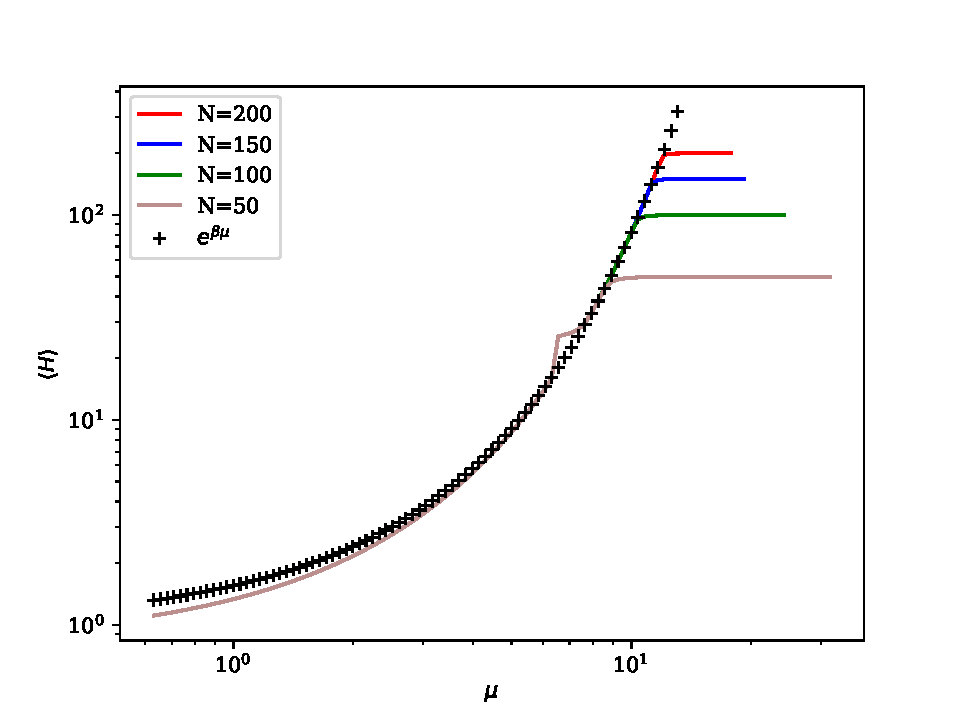
\includegraphics[width=0.5\linewidth]{isingtosos/hauteur-tm-pop.pdf}
	\caption{Position d'équilibre de l'interface \ref{tm-magnetisation} en fonction de $\mu$ via diagonalisation de la matrice de transfert \ref{hamil-pop}. Plus $\mu$ augmente, et plus la formule analytique \ref{position-hauteur-pop} via la formule de Stirling est valable (en pointillés).}
	\label{figure-pop}
\end{figure}
	
Lorsque nous avons fait l'approximation SOS dans le modèle d'Ising, nous sommes passés d'un système où l'on prenait en compte toutes les interactions entre particules vers un modèle d'interface où seul comptent les particules au niveau de l'interface, perdant ainsi l'information sur le bulk. Chaque site $i$ est maintenant définit par la coordonnée de la hauteur de l'interface $h_i$, dont l'entropie est donnée par les permutations possibles des hauteurs.
Nous proposons ici un nouveau modèle, où nous n'avons pas perdu l'information sur la position des particules, que nous nommerons \textbf{le modèle Particles-Over-Particles} (POP). Soit $N = \sum_i h_i$ le nombre de spins $+$ dans le système, c'est-à-dire l'aire sous l'interface.
La grande fonction de partition devient
\begin{align}
    \Xi(\mu) = \sum_{{\bf h_i }} e^{- \beta J \sum_{i} |h_i-h_{i+1}| + \beta \mu \sum_i h_i  - \sum_i \ln(h_i !)} 
    \label{hamil-pop}
\end{align}
où le second terme provient du fait qu'il y a $N! / \Pi_i h_i! $ manières de choisir les configurations spécifiées par les $h_i$ parmi les $N = \sum_i h_i$ particules qui sont indiscernables entre elles. 
Le potentiel effectif contient le potentiel chimique ainsi que l'effet de l'entropie
\begin{align}
    V_e = \beta \mu \sum_i h_i - \sum_i \ln(h_i!)
\end{align}
Grâce à la formule de Stirling pour $h_i$ grand, et en considérant une configuration où l'interface est lisse $h_i = <h>$, on a
\begin{align}
    \frac{dV}{d<h>} = 0 \rightarrow <h> = e^{\beta \mu} + C
    \label{position-hauteur-pop}
\end{align}
Dans la limite $\mu \to -\infty$, aucune particule ne peut se déposer dans le système, et donc $C=0$.



	\section{Particules indiscernables}
	Différence dans la fonction de partition en général


	\section{Avec le SOS}
	Le modèle Solid-On-Solid est l'approximation standard du modèle d'Ising car elle est étudiable analytiquement via sa matrice de transfert. 	Tout comme lorsque l'on déforme un flan seules les particules à l'interface flan-air peuvent bouger, dans le modèle SOS les particules loin de l'interface entre les deux phases ne peuvent bouger via l'agitation thermique. 
	Nous proposons alors un modèle un peu plus physique, dans lequel chaque particule a le droit de bouger. Au lieu de ne considérer que la hauteur $h_i$ au site $i$, nous considérons qu'il existe $h_i$ particules empilées les unes sur les autres. Lors d'un déplacement, nous prenons une particule au hasard pour la déplacer vers le haut de la pile, puis vers un autre site $j$. 
	Ainsi la fonction de partition devient
	
\begin{equation}
	Z = \sum_{h_1 h_2 ... h_L} e^{- \beta \sum_{i} H(i,i+1)} \frac{N!}{\prod_i n_i!} = N! \sum_{h_1 h_2 ... h_L} e^{- \beta \sum_{i} H(i,i+1) -\sum_i \ln(n_i!)}
\end{equation}

La matrice de transfert symétrisée devient donc
\begin{equation}
	T(h,h') = e^{-J |h-h'| - \frac{1}{2}(\ln(h!)-\ln(h'!)}
\end{equation}
où les termes $\ln(h)$ proviennent de l'entropie générée par la présence des particules au sein même des sites. À notre connaissance, ce modèle n'a pas été aussi étudié que le modèle SOS bien qu'il soit physiquement plus proche du modèle d'Ising initial. Le fait que la matrice de transfert ne soit pas résolvable analytiquement en est peut-être la cause. 
		\subsection{Modifications de l'algorithme Metropolis}
		au lieu de choisir un site, on choisit une particule, càd un site avec une proba pondérée.



	\section{Résultats modèle A}
	comment implémenter modèle A sur POP ? Différences avec SOS ?
	\section{Résultats modèle B}
	différences pour même hauteur moyenne, donner la distribution de hauteurs 
	on en déduit quoi ? 
	Mettre courbes de l'effet casimir, c'est pas mal
	\section{Résultats modèle A+B}
		certaines particules soumises à A, certaines à B. 